\documentclass{beamer}

\usepackage{polski}
\usepackage[utf8x]{inputenc}
\usepackage{minted}

\usetheme{CambridgeUS}
%\usecolortheme{crane}

% Minted configuration
\setminted{frame=single}
\setminted[html]{linenos=true}

% On each section, add extra slide with section name
\AtBeginSection[]{
  \begin{frame}
    \vfill
    \centering
    \begin{beamercolorbox}[sep=10pt,center]{title}
      \usebeamerfont{title}\insertsectionhead\par
    \end{beamercolorbox}
    \vfill
  \end{frame}
}

\title{WebAcademy --- JavaScript}
\author{Adam Taciak}
\institute{Fujitsu (PTECH)}
\date{Styczeń 2021}


\begin{document}

\frame{\titlepage}

\section{Wprowadzenie}


\begin{frame}[fragile]
  \frametitle{Wprowadzenie}
  \framesubtitle{Informacje ogólne}

  Język \textbf{JavaScript}:
  \begin{itemize}
    \item początkowo powstał w celu "ożywienia" statycznych stron internetowych
    \item jest językiem skryptowym
    \item można uruchamiać wewnątrz przeglądarki internetowej
    \item nie należy łączyć go z językiem \textbf{Java}
  \end{itemize}
\end{frame}


\begin{frame}[fragile]
  \frametitle{Wprowadzenie}
  \framesubtitle{Informacje ogólne}

  Język \textbf{JavaScript} dzisiaj:
  \begin{itemize}
    \item w pierwszej dziesiątce najpopularniejszych języków programowania*
    \item możliwość uruchamiania poza środowiskiem przeglądarki internetowej
  \end{itemize}

  \textit{* według indeksu TIOBE}
\end{frame}


\begin{frame}[fragile]
  \frametitle{Wprowadzenie}
  \framesubtitle{Możliwości języka}

  Co \textbf{JavaScript} może zrobić w środowisku przeglądarki:
  \begin{itemize}
    \item dodawać, usuwać, modyfikować kod HTML
    \item dodawać, modyfikować style
    \item reagować na akcje użytkownika (klikanie, ruch myszą)
    \item wysyłać zapytania do zewnętrznych serwerów
    \item ustawiać i czytać ciasteczka (ang. cookies)
    \item przechowywać dane po stronie klienta
  \end{itemize}
\end{frame}


\begin{frame}[fragile]
  \frametitle{Wprowadzenie}
  \framesubtitle{Możliwości języka}

  Czego \textbf{JavaScript} nie może zrobić w środowisku przeglądarki:
  \begin{itemize}
    \item czytać/modyfikować plików systemu operacyjnego
    \item komunikacja z innymi zakładkami/oknami jest ograniczona
    \item odbieranie danych z innych domen jest ograniczone
  \end{itemize}
\end{frame}


\begin{frame}[fragile]
  \frametitle{Wprowadzenie}
  \framesubtitle{Podsumowanie}

  \begin{itemize}
    \item język \textbf{JavaScript} powstał z myślą o działaniu w przeglądarkach internetowych
    \item w przeszłości: \textbf{JavaScript} -- front-end, \textbf{PHP}, \textbf{Python}, \textbf{Java} -- back-end
    \item obecnie również back-end powstaje w języku \textbf{JavaScript}
  \end{itemize}
\end{frame}







\section{Pierwszy program}


\begin{frame}[fragile]
  \frametitle{Pierwszy program}
  \framesubtitle{Witaj świecie!}

  \begin{minted}{html}
<html>
  <body>
    <script>
      alert('Witaj świecie!');
    </script>
  </body>
</html>
  \end{minted}

\end{frame}




\section{Narzędzia programisty}

\begin{frame}[fragile]
  \frametitle{Narzędzia programisty}
  \framesubtitle{Wprowadzenie}

  Współczesne przeglądarki internetowe, posiadają wbudowane narzędzia, które pomagają w pracy programisty.

  \begin{itemize}
    \item inspektor drzewa DOM/stylów
    \item konsolę Web
    \item debugger
    \item podgląd \verb|local storage|, ciasteczek
    \item i inne
  \end{itemize}

  Dla nas, najciekawszym narzędziem będzie konsola.
\end{frame}


\begin{frame}[fragile]
  \frametitle{Narzędzia programisty}
  \framesubtitle{Wprowadzenie}

  Aby uruchomić narzędzia dla progamisty, należy w oknie przeglądarki wcisnąć przycisk \textbf{F12}.
\end{frame}


\begin{frame}[fragile]
  \frametitle{Narzędzia programisty}
  \framesubtitle{Firefox}

  \begin{figure}
    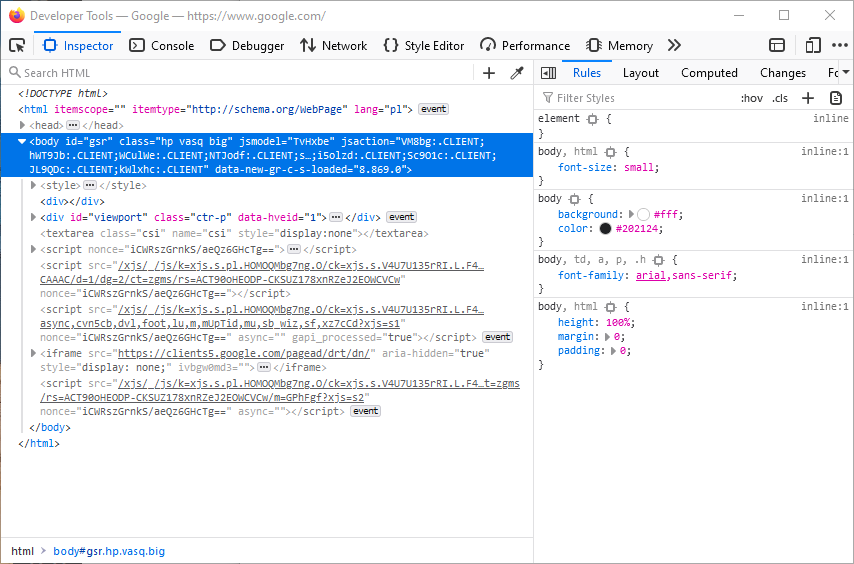
\includegraphics[scale=0.45]{images/dev-tools-firefox}
  \end{figure}

\end{frame}


\begin{frame}[fragile]
  \frametitle{Narzędzia programisty}
  \framesubtitle{Chrome}

  \begin{figure}
    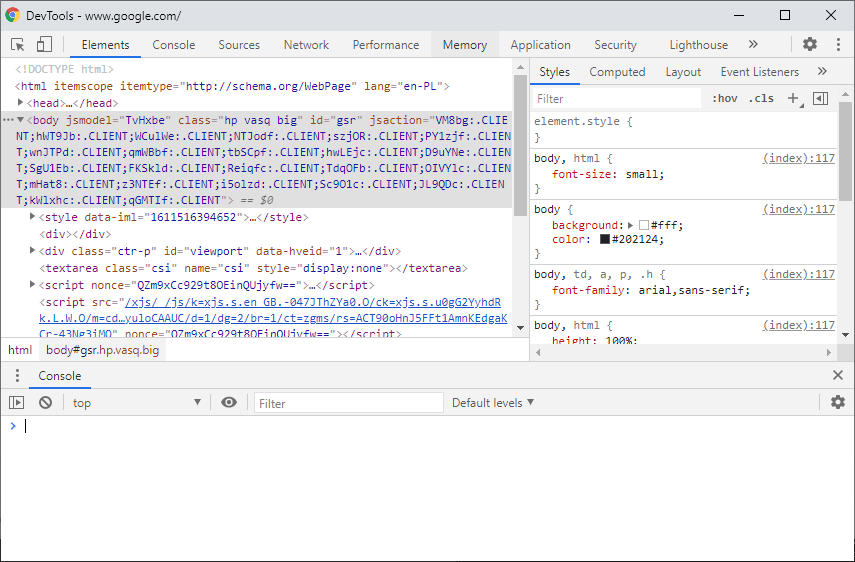
\includegraphics[scale=0.45]{images/dev-tools-chrome}
  \end{figure}
\end{frame}


\begin{frame}[fragile]
  \frametitle{Narzędzia programisty}
  \framesubtitle{Konsola}

  Konsola daje dostęp do interpretera języka \textbf{JavaScript}.

  \begin{itemize}
      \item podgląd błędów
      \item wywoływanie istniejącego kodu (funkcje)
      \item tworzenie zmiennych, funkcji
  \end{itemize}

  Jednak takie operacje nie są trwałe!
\end{frame}


\begin{frame}[fragile]
  \frametitle{Narzędzia programisty}
  \framesubtitle{Konsola}

  \begin{figure}
    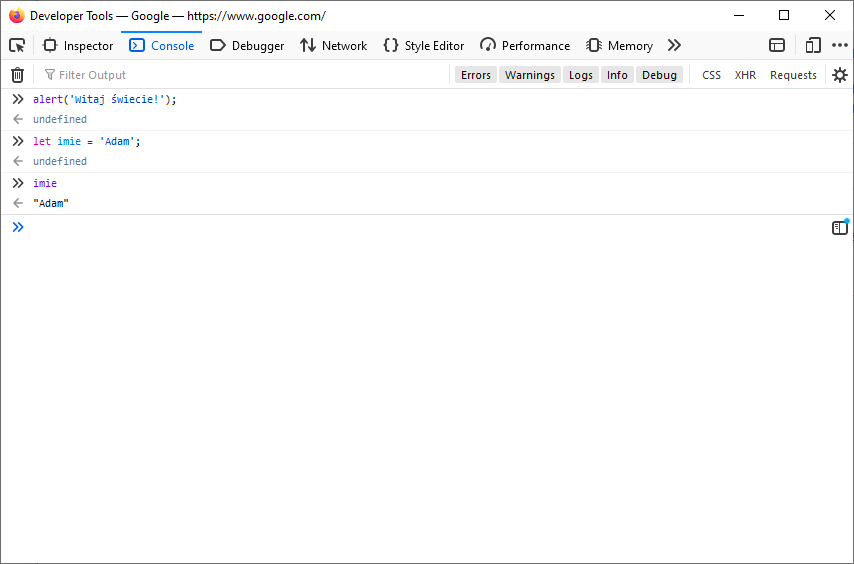
\includegraphics[scale=0.45]{images/dev-tools-console}
  \end{figure}
\end{frame}


\begin{frame}[fragile]
  \frametitle{Narzędzia programisty}
  \framesubtitle{Obiekt console}

  W trakcie tworzenia aplikacja, pojawia się potrzeba logwania róznych zdarzeń. Do tego celu służy obiekt \verb|console|.

  {\footnotesize
    \begin{itemize}
      \item \verb|console.log(obj1 [,obj2, ..., objN])| --- logowanie
      \item \verb|console.warn(obj1 [,obj2, ..., objN])| --- ostrzeżenie
      \item \verb|console.info(obj1 [,obj2, ..., objN])| --- informacja
      \item \verb|console.error(obj1 [,obj2, ..., objN])| --- błąd
    \end{itemize}
  }
\end{frame}


\begin{frame}[fragile]
  \frametitle{Narzędzia programisty}
  \framesubtitle{Obiekt console}

  Wszystkie metody działają bardzo podobnie. Wyświetlają przekazany argument w konsoli:

  \begin{minted}{js}
console.log('Ala ma kota');
console.info('Ala', 'ma', 'kota');
console.warn('Ala ma', 14, 'lat');
console.error('Kot ma Alę');
  \end{minted}

  \begin{figure}
    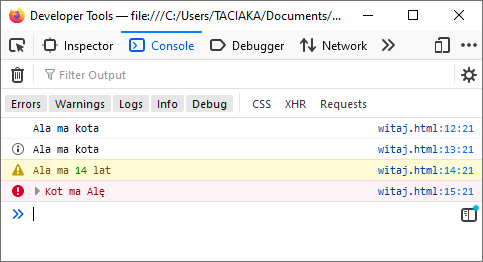
\includegraphics[scale=0.45]{images/dev-tools-console-example}
  \end{figure}


\end{frame}




\section{Zmienne}

\begin{frame}[fragile]
  \frametitle{Zmienne}
  \framesubtitle{Definicja}

  \textbf{Zmienna} (ang. variable) jest magazynem z nazwą dla danych.

  \begin{itemize}
    \item służą do przechowywania danych
    \item podobnie jak w języku \textbf{Python} ich typ jest dynamiczny
    \item deklaracja zmiennej przez słowo kluczowe \verb|let|
  \end{itemize}

  \begin{minted}{js}
    let imie;
    let wiek = 15;
  \end{minted}
\end{frame}


\begin{frame}[fragile]
  \frametitle{Zmienne}
  \framesubtitle{Definicja}

  Nazwa zmiennej ma pewne ograniczenia:

  \begin{itemize}
    \item moża zawierać tylko: litery, cyfry oraz znaki \$ \_
    \item pierwszym znakiem nie może być cyfra
  \end{itemize}
\end{frame}

\begin{frame}[fragile]
  \frametitle{Zmienne}
  \framesubtitle{Definicja}

  Prawidłowe nazwy zmiennych:
  \begin{minted}{js}
    let imie;
    let $nazwisko;
    let zmienna123;
    let login_lub_haslo;
    let nazwaUzytkownika;
  \end{minted}
\end{frame}


\begin{frame}[fragile]
  \frametitle{Zmienne}
  \framesubtitle{Definicja}

  Nieprawidłowe nazwy zmiennych:
  \begin{minted}{js}
    let 1imie;
    let imie nazwisko;
    let wiek%;
  \end{minted}
\end{frame}

\begin{frame}[fragile]
  \frametitle{Zmienne}
  \framesubtitle{Definicja}

  Nazwy zmiennych mogą posiadać polskie znaki:

  \begin{minted}{js}
    let imię;
    let czyObowiązkowy;
    let prędkość_maksymalna;
  \end{minted}

  \textbf{Ale uwaga! Dobrą praktyką jest unikanie używania polskich znaków.}
\end{frame}


\begin{frame}[fragile]
  \frametitle{Zmienne}
  \framesubtitle{Definicja}

  Deklaracja zmiennej odbywa się przy użyciu słowa kluczowego \verb|let|:

  \begin{minted}{js}
    let mojaZmienna;
  \end{minted}

  W trakcje deklaracji, zmienną możemy inicjalizować wartością przy użyciu operatora przypisania \verb|=|:

  \begin{minted}{js}
    let mojaZmienna = 'Ala ma kota';

    let mojaZmienna;
    mojaZmienna = 'Ala ma kota';
  \end{minted}
\end{frame}


\begin{frame}[fragile]
  \frametitle{Zmienne}
  \framesubtitle{Definicja}

  Ponowne przypisanie wartości do zmiennej, powoduje nadpisanie poprzedniej wartości:

  \begin{minted}{js}
    let mojaZmienna = 'Ala ma kota';  // Ala ma kota
    mojaZmienna = 'Ala ma psa';       // Ala ma psa
    mojaZmienna = 123;                // 123
  \end{minted}

\end{frame}


\begin{frame}[fragile]
  \frametitle{Zmienne}
  \framesubtitle{Definicja}

  Informacje powiązane ze zmiennymi, które w tej chwili pominiemy:

  \begin{itemize}
      \item słowo kluczowe \verb|var|
      \item zasięg zmiennych
  \end{itemize}
\end{frame}


\begin{frame}[fragile]
  \frametitle{Zmienne}
  \framesubtitle{Definicja}

  \verb|prompt(message, default)| --- wyświetla okno dialogowe do wprowadzania tekstu, zwraca wprowadzony tekst

  \begin{itemize}
      \item \verb|message| --- komunikat wyświetlany w oknie dialogowym 
      \item \verb|default| --- wartość domyślna pola 
  \end{itemize}
  
  \begin{minted}{js}
    let imie = prompt('Jak masz na imię?');
  \end{minted}

  \begin{figure}
    
\includegraphics[scale=0.5]{images/js-prompt-example}
  \end{figure}
\end{frame}


\section{Typy danych}

\begin{frame}[fragile]
  \frametitle{Typy danych}
  \framesubtitle{Wprowadzenie}

  Wartość w języku \textbf{JavaScript} zawsze ma określony typ. 

  \begin{itemize}
    \item \verb|number| --- liczby
    \item \verb|bigInt| --- duże liczby
    \item \verb|string| --- ciągi znakowe
    \item \verb|boolean| --- wartość prawda/fałsz
    \item wartosć \verb|null| --- wartość pusta
    \item wartość \verb|undefined| --- wartość niezainicjalizowana
    \item \verb|object| --- objekt
  \end{itemize}

\end{frame}

\begin{frame}[fragile]
  \frametitle{Typy danych}
  \framesubtitle{number}

 Typ \verb|number| przechowuje liczbę:

  \begin{minted}{js}
let liczba_a = 123;
let liczba_b = 12.3; 
  \end{minted}

\end{frame}


\begin{frame}[fragile]
  \frametitle{Typy danych}
  \framesubtitle{number}

 Na typie \verb|number| można wykonywać operacje matematyczne:

  \begin{minted}{js}
let a = 10 + 2;
let b = 20 - 2;
let c = 5 * 5;
let d = 16 / 8;
  \end{minted}

\end{frame}


\begin{frame}[fragile]
  \frametitle{Typy danych}
  \framesubtitle{string}

 Typ \verb|string| przechowuje łańcuch znakowy:

  \begin{minted}{js}
let napis_a = 'Ala ma kota';
let napis_b = "Ala ma psa";
let napis_c = `Ala ma chomika`;
  \end{minted}

\end{frame}


\begin{frame}[fragile]
  \frametitle{Typy danych}
  \framesubtitle{string}

 Na typie \verb|string| można wykonywać operację konkatenacji (łączenia):

  \begin{minted}{js}
let napis = 'Ala ' + 'ma' + ' kota';
  \end{minted}

\end{frame}

\begin{frame}[fragile]
  \frametitle{Typy danych}
  \framesubtitle{boolean}

 Typ \verb|boolean| przechowuje informację prawdwa/fałsz:

  \begin{minted}{js}
let prawda = true;
let falsz = false;
  \end{minted}

\end{frame}


\begin{frame}[fragile]
  \frametitle{Typy danych}
  \framesubtitle{string}

 Typ \verb|boolean| najczęściej będziemy używać przy konstrukcjach warunkowych:

  \begin{minted}{js}
let czyPelnoletni = false;
if (czyPelnoletni) {
  alert('Użytkownik jest pełnoletni');
}
  \end{minted}

\end{frame}


\begin{frame}[fragile]
  \frametitle{Typy danych}
  \framesubtitle{null}

 Wartość \verb|null| oznacza nic, brak danych:

  \begin{minted}{js}
let napis = null;
  \end{minted}

  Zmienna \verb|napis| przechowuje informację o braku informacji.

\end{frame}


\begin{frame}[fragile]
  \frametitle{Typy danych}
  \framesubtitle{undefined}

 Wartość \verb|undefined| oznacza, iż zmienna pozostaje niezainicjalizowana:

  \begin{minted}{js}
let napis;
console.log(napis);
  \end{minted}

  Zmienna \verb|napis| została zadeklarowana, jednak jej początkowa wartość pozostaje nieokreślona.

\end{frame}


\begin{frame}[fragile]
  \frametitle{Typy danych}
  \framesubtitle{object}

 Typ \verb|object| jest typem złożonym

  \begin{minted}{js}
let samochod = {
  marka: 'Porsche',
  model: '911 Turbo',
  predkoscMax: 210
}
  \end{minted}

  Zmienna \verb|samochod| reprezentuje obiekt zbudowany z 3 pól (typów prostych).

\end{frame}

%\input{06-data-conversions}
\section{Zdarzenia HTML}

\begin{frame}[fragile]
  \frametitle{Zdarzenia}
  \framesubtitle{Wprowadzenie}

  \textbf{HTML} posiada zestaw zdarzeń które mogą wywoływać kod \textbf{JavaScript}

  \begin{itemize}
    \item zdarzenia okna (\verb|onload|, \verb|onresize|)
    \item zdarzenia formularzy (\verb|onfocus|, \verb|onsubmit|)
    \item zdarzenia klawiatury (\verb|onkeydown|, \verb|onkeyup|)
    \item zdarzenia myszy (\verb|onclick|, \verb|onwheel|)
    \item zdarzenia przenoszenia (\verb|ondrag|, \verb|ondrop|)
    \item zdarzenia schowka (\verb|oncopy|, \verb|onpaste|)
  \end{itemize}

\end{frame}


\begin{frame}[fragile]
  \frametitle{Zdarzenia}
  \framesubtitle{Wprowadzenie}

  Zdarzenia zezwalają na wykonywanie kodu \textbf{JavaScript} w interakcji z użytkownikiem:

  \begin{itemize}
    \item (Z) po pełnym załadowaniu strony, (JS) wyświetl komunikat
    \item (Z) kliknięcie w przycisk, (JS) zmienia kolor strony
    \item (Z) po najechaniu kursorem na zdjęcie, (JS) powiększ je
  \end{itemize}
\end{frame}


\begin{frame}[fragile]
  \frametitle{Zdarzenia}
  \framesubtitle{Wprowadzenie}

  Przykład użycia:

  \begin{minted}{html}
<button onclick="alert('Witaj świecie')">
</button>
  \end{minted}

\end{frame}


\section{Selektory DOM}

\begin{frame}[fragile]
  \frametitle{Selektory DOM}
  \framesubtitle{Wprowadzenie}

  Model \textbf{DOM} jest obiektowym sposobem reprezentowania dokumentu \textbf{HTML}.

  \begin{itemize}
    \item definiuje klasy i interfejsy dostępu do elementów
    \item oraz mechanizmy tworzenia/usuwania węzłów
    \item istnieją gotowe biblioteki do obsługi
  \end{itemize}

\end{frame}

\begin{frame}[fragile]
  \frametitle{Selektory DOM}
  \framesubtitle{Wprowadzenie}

  \begin{figure}
    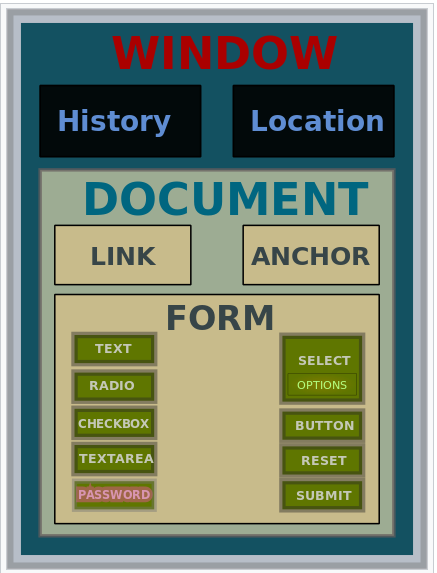
\includegraphics[scale=0.45]{images/dom-structure}
  \end{figure}

\end{frame}

\begin{frame}[fragile]
  \frametitle{Selektory DOM}
  \framesubtitle{Selektory}

  \verb|JavaScript| posiada wbudowane selektory drzewa DOM:

  \begin{itemize}
    \item \verb|getElementById(id)| --- zwraca element o podanym id
    \item \verb|getElementsByTagName(name)| --- zwraca listę elementów o podanym tagu
    \item \verb|getElementsByClassName(name)| --- zwraca listę elementów po podanej klasie
  \end{itemize}

\end{frame}


\begin{frame}[fragile]
  \frametitle{Selektory DOM}
  \framesubtitle{Selektory}

  Przykłady użycia zostaną przedstawione na podstawie następującegu kodu:

  \begin{minted}{html}
<html>
    <body>
        <h1 id="tytul">Witaj świecie</h1>
        <ol>
            <li class="czarny">Hello world</li>
            <li class="szary">Hallo Welt!</li>
            <li class="czarny">Bonjour le monde!</li>
        </ol>
    </body>
</html>
  \end{minted}

\end{frame}

\begin{frame}[fragile]
  \frametitle{Selektory DOM}
  \framesubtitle{Selektory}

  \begin{figure}
    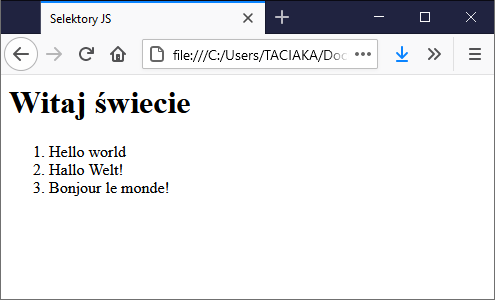
\includegraphics[scale=0.75]{images/dom-selectors-example}
  \end{figure}

\end{frame}


\begin{frame}[fragile]
  \frametitle{Selektory DOM}
  \framesubtitle{Selektory}

  \verb|document.getElementById(id)| --- zwraca obiekt o podanym identyfikatorze lub \verb|null|

  \begin{minted}{js}
let naglowek = document.getElementById('tytul');
  \end{minted}

  \begin{figure}
    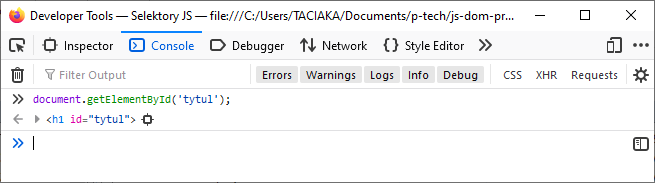
\includegraphics[scale=0.55]{images/dom-selector-getelementbyid}
  \end{figure}

\end{frame}


\begin{frame}[fragile]
  \frametitle{Selektory DOM}
  \framesubtitle{Selektory}

  \verb|document.getElementsByClassName(name)| --- zwraca listę obiektów o podanej klasie lub pustą listę

  \begin{minted}{js}
let czarne = document.getElementsByClassName('czarny');
  \end{minted}

  \begin{figure}
    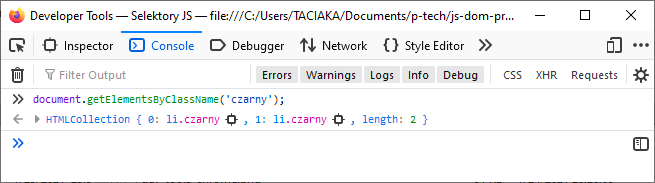
\includegraphics[scale=0.55]{images/dom-selector-getelementsbyclassname}
  \end{figure}

\end{frame}


\begin{frame}[fragile]
  \frametitle{Selektory DOM}
  \framesubtitle{Selektory}

  \verb|document.getElementsByTagName(name)| --- zwraca listę obiektów o podanym tagu lub pustą listę

  \begin{minted}{js}
let elementy = document.getElementsByTagName('li');
  \end{minted}

  \begin{figure}
    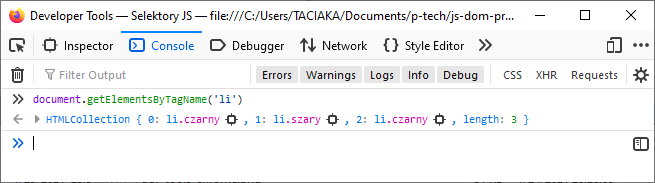
\includegraphics[scale=0.55]{images/dom-selector-getelementsbytagname}
  \end{figure}

\end{frame}


\begin{frame}[fragile]
  \frametitle{Selektory DOM}
  \framesubtitle{Obiekt HTMLElement}

  W zasadzie do czego przyda się zwracany element?

  Selektory zwracają obiekt \verb|HTMLElement| lub \verb|HTMLCollection| które reprezentują elementy w kodzie \textbf{HTML}.

  \begin{itemize}
    \item przez zwrócony obiekt, można rozmawiać z elementem na stronie
    \item atrybuty obiektu są odwzorowaniem atrybutów w HTMLu
  \end{itemize}

\end{frame}


\begin{frame}[fragile]
  \frametitle{Selektory DOM}
  \framesubtitle{Obiekt HTMLElement}

  Przykład:

  Kod \textbf{HTML}
  \begin{minted}{html}
<h1 id="tytul">Witaj świecie!<h1>
  \end{minted}

Kod \textbf{JavaScript}
  \begin{minted}{js}
let element = document.getElementById('tytul');
console.log(element.innerText);
  \end{minted}

Wyjście w konsoli
  \begin{minted}{bash}
Witaj świecie
  \end{minted}

\end{frame}


\begin{frame}[fragile]
  \frametitle{Selektory DOM}
  \framesubtitle{Obiekt HTMLElement}

  Co \verb|HTMLElement| kryje w sobie:

  \begin{itemize}
    \item \verb|innerText| --- tekst przechowywany w elemencie
    \item \verb|innerHTML| --- HTML przechowywany w elemencie
    \item \verb|hidden| --- ukrycie elementu
    \item \verb|id| --- identyfikator elementu
    \item \verb|className| --- klasa elementu
    \item \verb|style| --- dostęp do stylu elementu
    \item \verb|value| --- wartość elementu (pola tekstowe)
  \end{itemize}

\end{frame}


\begin{frame}[fragile]
  \frametitle{Selektory DOM}
  \framesubtitle{Obiekt HTMLElement}

  A jak modyfikować styl elementu?

  Aby zrealizować poniższy styl:
  \begin{minted}{css}
#tytul {
  color: red;
  font-size: 20px;
}
  \end{minted}

Należy odwołać się do poszczególnych atrybutów:
  \begin{minted}{js}
let element = document.getElementById('tytul');
element.style.color = 'red';
element.style.fontSize = 20;
  \end{minted}

\end{frame}










\end{document}
